%! TEX root = **/000-main.tex
% vim: spell spelllang=en:

\section{Extrapolation}%
\label{sec:extrapolation}

It is crucial that we choose an extrapolation method which benifits from the specific properties of our system and solver.
Due to the time constraint on this project we haven't investigated the stability or error bound properties for the extrapolation methods.
While this would be an interesting area to do further research in, we chose methods for which we can safely ignore these properties.
Neuro-VISOR uses the Semi-Implicit Backward Difference 2 method\cite{neuroVISOR}, so linear and quadratic extrapolation are both good options.
To minimize the runtime and memory usage of the extrapolation we've chosen to implement linear extrapolation.

\begin{figure}[H]
    \centering
    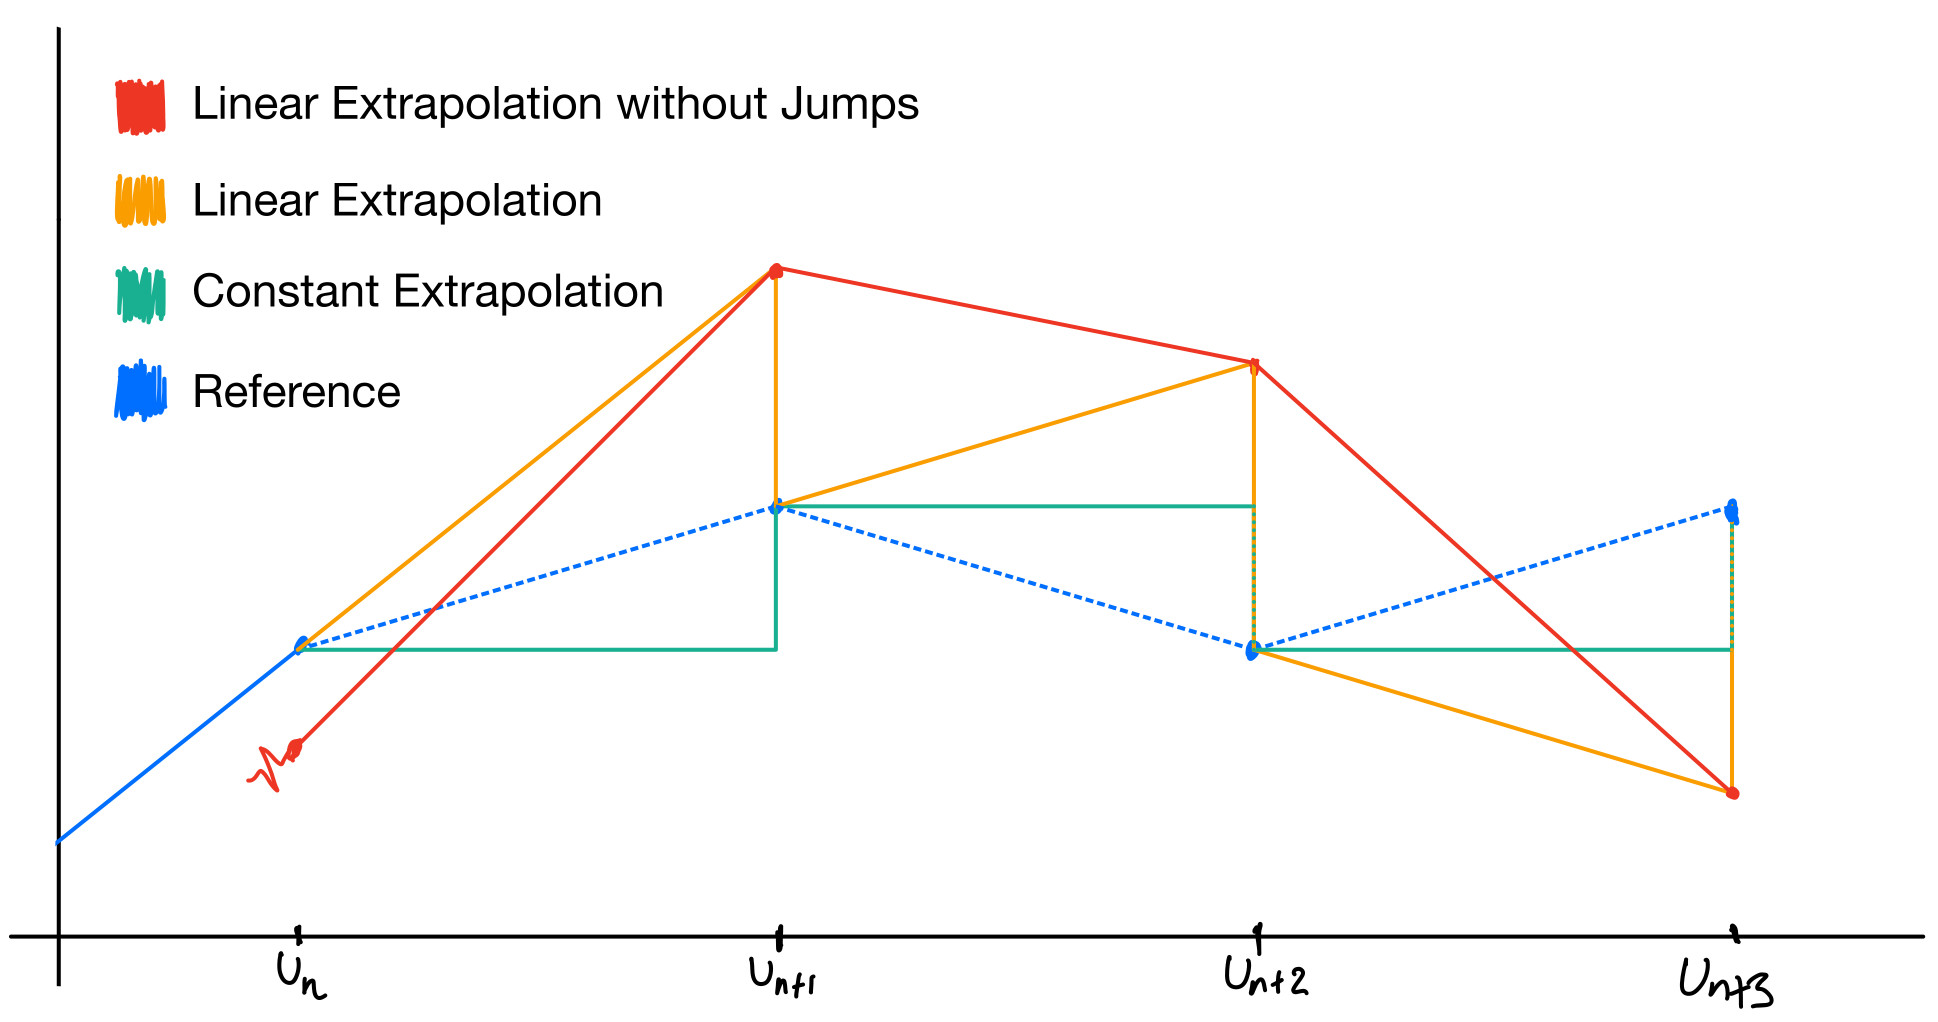
\includegraphics[width=1.0\linewidth]{extrapolationOptions}
    \caption{Linear Extrapolation Methods}%
    \label{fig:extrapMethods}
\end{figure}

Linear extrapolation requires a linear function defined in terms of the previous data points.
As seen in \cref{fig:extrapMethods}, there are multiple ways of defining the linear function.
The naive way would be to use the constant function equal to the most recent data point.
An example of this can be seen in \cref{fig:extrapMethods} as the green option.
Technically Neuro-VISOR implements this as the visualization updates more frequently than the simulation.
Another option is to use the tangent line defined by the previous two data points.
This corresponds to the yellow option in \cref{fig:extrapMethods}.
Yet another option is to use the slope between the previous two data points and the point along the previous extrapolation which coincides with the time of the most recent data point.
This can be seen in \cref{fig:extrapMethods} as the red option.

As mentioned in the introduction, the goal of this project is to improve the visualization and user experience of the program during unexpected slow downs.
While this is not rigorously definied, we will suppose abrupt jumps decrease the user's experience.
This seems like a reasonable heuristic, as abrupt jumps are jarring and make it difficult to follow the simulation.
The naive line results in a jump whenever a new data point is calculated unless the system is constant.
The tangent line also results in a similar number of jumps, but the jumps will generally be smaller than the naive line.
Because of this, the tangent line is strictly better for our use case.
The last option doesn't contain any jumps.
However, since it doesn't jump to the most recent data point the error bounds accumulate.
There are ways of defining the extrapolation line to account for this.
For example, one could cap the distance between the point used and the previous data point.
Another way could be to define the slope using both the tangent slope and the distance between the starting point and previous data point.
While this is an interesting avenue for further research, we will use this definition with the assumption that the error bounds won't cause any issues.
Experimentally, Neuro-VISOR's time step is small enough for the error bounds to be negligably small\cite{neuropy}.
With all of this information,  we should choose the tangent line when emphasizing the accuracy and the third option when emphasizing the user experience.
To get a more hands on understanding of the two linear function definitions we have implmented them in neuropy.
